\section{ПРАКТИЧЕСКАЯ ЧАСТЬ}


\subsection{Используемые инструменты}

\begin{itemize}
 \item Python 3


 \item NumPy


 \item Pandas


 \item Matplotlib



 \item Pymorphy2


 \item Razdel



 \item TensorFlow



 \item Scikit-learn



 \item JavaScript


 \item HTML и CSS



\end{itemize}














\subsection{Сбор данных}


Самым главным этапом перед созданием моделей-классификаторов является сбор данных, этот процесс включает в себя несколько основных этапов:

\bigskip
\begin{itemize}
 \item обработка и подготовка текстов;
 \item разметка текстов;
 \item обработка полученных результатов.
\end{itemize}

\subsubsection{Обработка и подготовка текстов}

В качестве основного текста для разметки был взят роман Михаила Афанасьевича Булгакова <<Мастер и Маргарита>>.

\bigskip
Обработка документа:

\bigskip
\begin{enumerate}
\item произведение было очищено от нежелательных подстрок регулярными выражениями;
\item разделено на тексты по символу перевода строки <<\textbackslash n>>;
\item из полученных текстов восстановлена прямая речь;
\item тексты содержащие больше 52 слов разделены с использованием библиотеки <<razdel>>.
\end{enumerate}

\bigskip
Формирование заданий:

\bigskip
\begin{itemize}
 \item для разметки выделены тексты от 5 до 52 слов;
 \item для каждого текста определен контекст:  не менее 40 слов перед и не менее 15 после текста.
\end{itemize}



\subsubsection{Разметка текстов}

Чтобы приступить к разметке сначала нужно определить множество меток классов, для этого обратимся к истории создания эмоциональных моделей ведушими профессорами в области изучения эмоций. В 1980 году Роберт Плутчик в своей работе \cite{Plutchik} определил колесо эмоций рис. \ref{fig:plutchik}. Данная модель была взята за основу и дополнена моделью Пола Экмана, которую он описал в работе \cite{Ekman2004} 2004 года и обновил в статье \cite{Ekman2011} 2011 года.

\begin{figure}[ht]
    \centering
    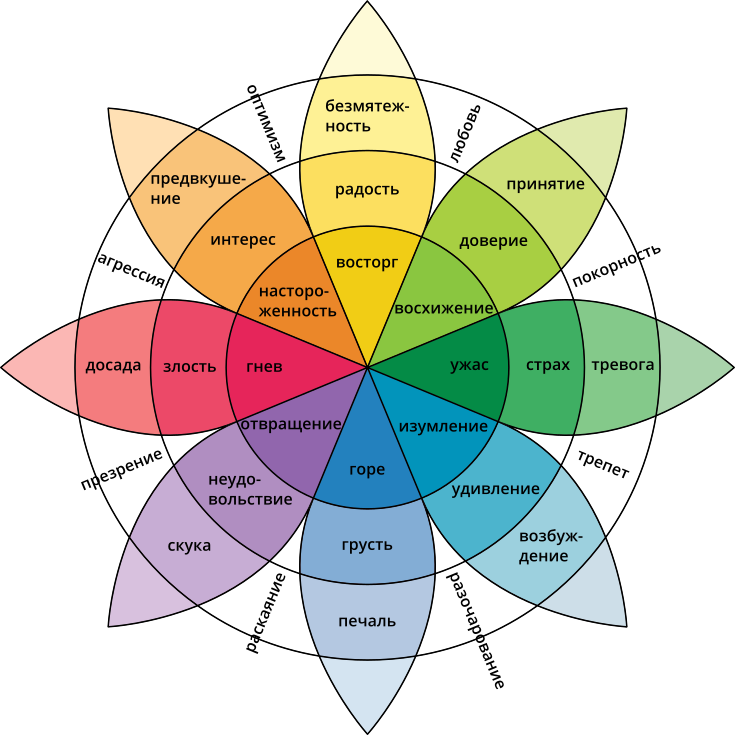
\includegraphics[scale=0.5]{plutchik.png}
    \caption{Колесо эмоции Роберта Плутчика}
    \label{fig:plutchik}
\end{figure}

В результате получилось множество, состоящее из 9 основных эмоций и их производных, дополненное нейтральным классом:

\bigskip
\begin{itemize}
\item \textbf{Злость} (anger) --- желание выразить агрессию или причинить зло, общая для обеих моделей.\\
Может проявляться в словах, мимике, поступках.
Примеры: злость на оскорбление, на несправедливость, злость на плохое отношение.\\
Гнев --- более интенсивная эмоция, досада --- менее.

\item \textbf{Интерес} (anticipation) --- предчувствие важного события, только в модели Плутчика.\\
Проявляется в нетерпении, волнении.
Примеры: ожидание праздника, ожидание начала каникул, ожидание плохой оценки.\\
Настороженность --- более интенсивная, предвкушение --- менее.

\item \textbf{Радость} (joy) --- чувство удовольствия, весёлого настроения и счастья, общая для обеих моделей.\\
Проявляется в смехе, улыбке, ласковом обращении к другим.
Примеры: радость по поводу подарка, общения с другом.\\
Восторг --- более интенсивная, безмятежность --- менее.

\item \textbf{Доверие} (trust) --- ​открытое теплое отношение к чему бы то ни было (другу/животному/миру/...), только в модели Плутчика.\\
Проявляется в уверенности в положительном исходе.
Примеры: доверие другу при встрече с неожиданностями, доверие к собаке, что не укусит, доверие к доктору, что он делает полезные вещи.\\
Восхищение --- более интенсивная, принятие --- менее.

\item \textbf{Страх} (fear) --- состояние перед реальным или предполагаемым бедствием, общая для обеих моделей.\\
Проявляется в волнении, напряжении.
Пример: страх наказания, страх проигрыша, страх попасть в аварию.\\
Ужас --- более интенсивная, тревога --- менее.

\item \textbf{Удивление} (surprise) --- эмоциональная реакция на неожиданную ситуацию, общая для обеих моделей.\\
Удивление может проявляться в хороших и плохих ситуациях.
Примеры: получил плохой отзыв на работу вместо ожидаемого хорошего, директор школы привел в класс собаку, одноклассник вырос на 10 см за лето.\\
Изумление --- более интенсивная, возбуждение --- менее.


\item \textbf{Грусть} (sadness) --- отсутствие радости,​ неудовлетворенность происходящим, отстраненность, общая для обеих моделей.\\
Проявляется в нежелании веселиться с другими, желании заботы и участия.
Примеры: мама уехала в командировку надолго, не покупают собаку или велосипед, никак не дается математика.\\
Горе --- более интенсивная, печаль --- менее.

\item \textbf{Неудовольствие} (disgust) --- эмоциональная реакция на неприятную ситуацию или объект.\\
Проявляется в неприятии человека, любых вещей, ситуаций, общая для обеих моделей.
Примеры: когда сталкиваешься с неприятным запахом, грязными вещами, плохим поведением.\\
Отвращение --- более интенсивная, скука --- менее.

\item \textbf{Презрение} (contempt) --- пренебрежительное отношение к кому-чему-нибудь морально низкому, недостойному, подлому. Презрение связано с чувством превосходства. Также оно может перейти в безразличное отношение к кому-чему-то. Только в модели Экмана.

\item \textbf{Нейтральное} (neutral) --- безэмоциональное повествование.

\end{itemize}

\bigskip
Разметка осуществлялась с помощью краудсорсинговой платформы <<Яндекс.Толока>>.

\begin{definition}
 Краудсорсинг --- это привлечение добровольцев и экспетртов для выполнения определенной работы, действующих на добровольной или комерческой основе.
\end{definition}

Для получения более точной разметки данных были использованы встроенные методы и инструменты контроля качества:

\bigskip
\begin{itemize}
 \item график времени выполнения страницы заданий рис. \ref{fig:task-time} нужен, чтобы видеть на сколько вдумчиво эксперт расставляет метки;
 \item график выполнения заданий рис. \ref{fig:task-accept} показывает сколько выполнено страниц заданий, сколько просрочено и сколько пропущено. По нему можно судить о сложности выполнения задания и использовать эту информацию в процессе формирования новых пулов заданий;
 \item сформирована система правил, которая позволяет контролировать процесс разметки в автономном режиме:
    \medskip
    \begin{itemize}
     \item Eсли пропущенных подряд страниц заданий $\geqslant 10$, то заблокировать на проекте на $2$ дня;
     \item Eсли отправленных страниц заданий $\geqslant 50$, то заблокировать на проекте на $2$ дня;
     \item Минимальное время на страницу заданий --- $250$ сек. Учитывать последних страниц заданий --- $15$. Если количество ответов $\geqslant 5$ и количество быстрых ответов $\geqslant 5$, то заблокировать на проекте на $2$ дня и т.д.
    \end{itemize}
 \item размечены контрольные задания, с их помощью можно отслеживать примерную точность (accuracy), как всего набора данных, так и набора, полученного от одного эксперта;
 \item каждое задание выполняло три различных эксперта (перекрытие x3);
 \item агрегация результатов производилась методом Дэвида-Скина. Он автоматически оценивает для каждого исполнителя $|L|^2$ параметров, где $L$ --- множество возможных различных значений для агрегации и возвращает итоговый ответ и его статистическую значимость.
\end{itemize}


\begin{figure}[ht]
    \centering
    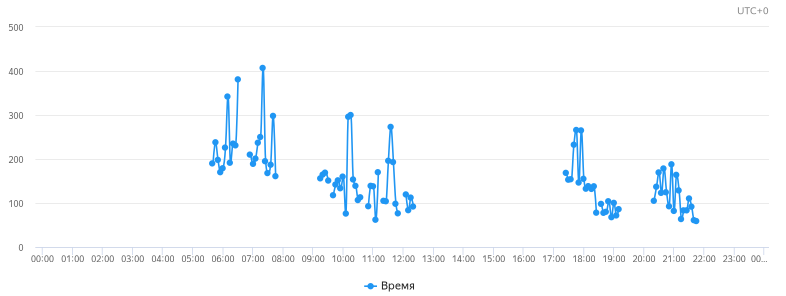
\includegraphics[scale=0.5]{task-time.png}
    \caption{Время выполнения страницы заданий (детализация по 5 минут)}
    \label{fig:task-time}
\end{figure}



\begin{figure}[ht]
    \centering
    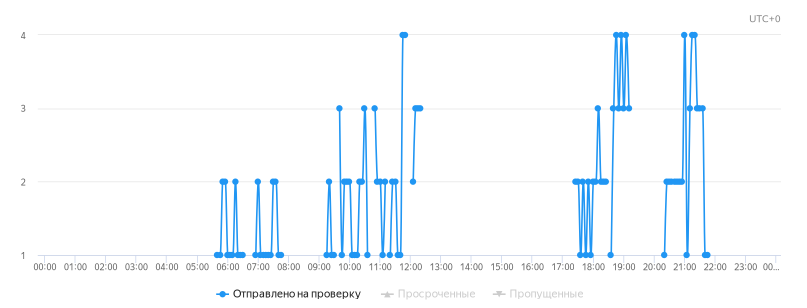
\includegraphics[scale=0.5]{task-accept.png}
    \caption{Выполнение страниц заданий (детализация по 5 минут)}
    \label{fig:task-accept}
\end{figure}

\bigskip
Была разработана форма задания рис. \ref{fig:task}. Каждое задание состоит из трех текстовых блоков. Страница заданий состоит из двух не размеченных заданий и одного контрольного, такое разбиение оптимально для получения качественных результатов. Эксперт должен прочитать каждый текстовый блок и отметить эмоции, которые, по его мнению, описаны в выделенном фрагменте.

\begin{figure}[ht]
    \centering
    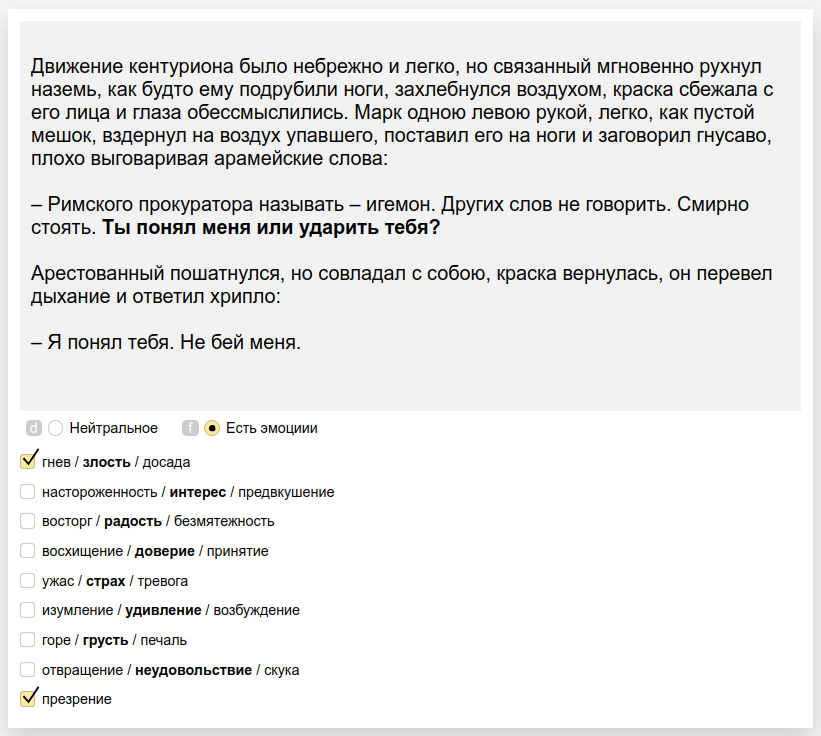
\includegraphics[scale=0.5]{task.png}
    \caption{Форма задания в сервисе <<Яндекс.Толока>>}
    \label{fig:task}
\end{figure}

\bigskip
В результате был сформирован набор данных с таким распределением классов рис. \ref{fig:class_distribution}.



\begin{figure}[ht]
    \centering
    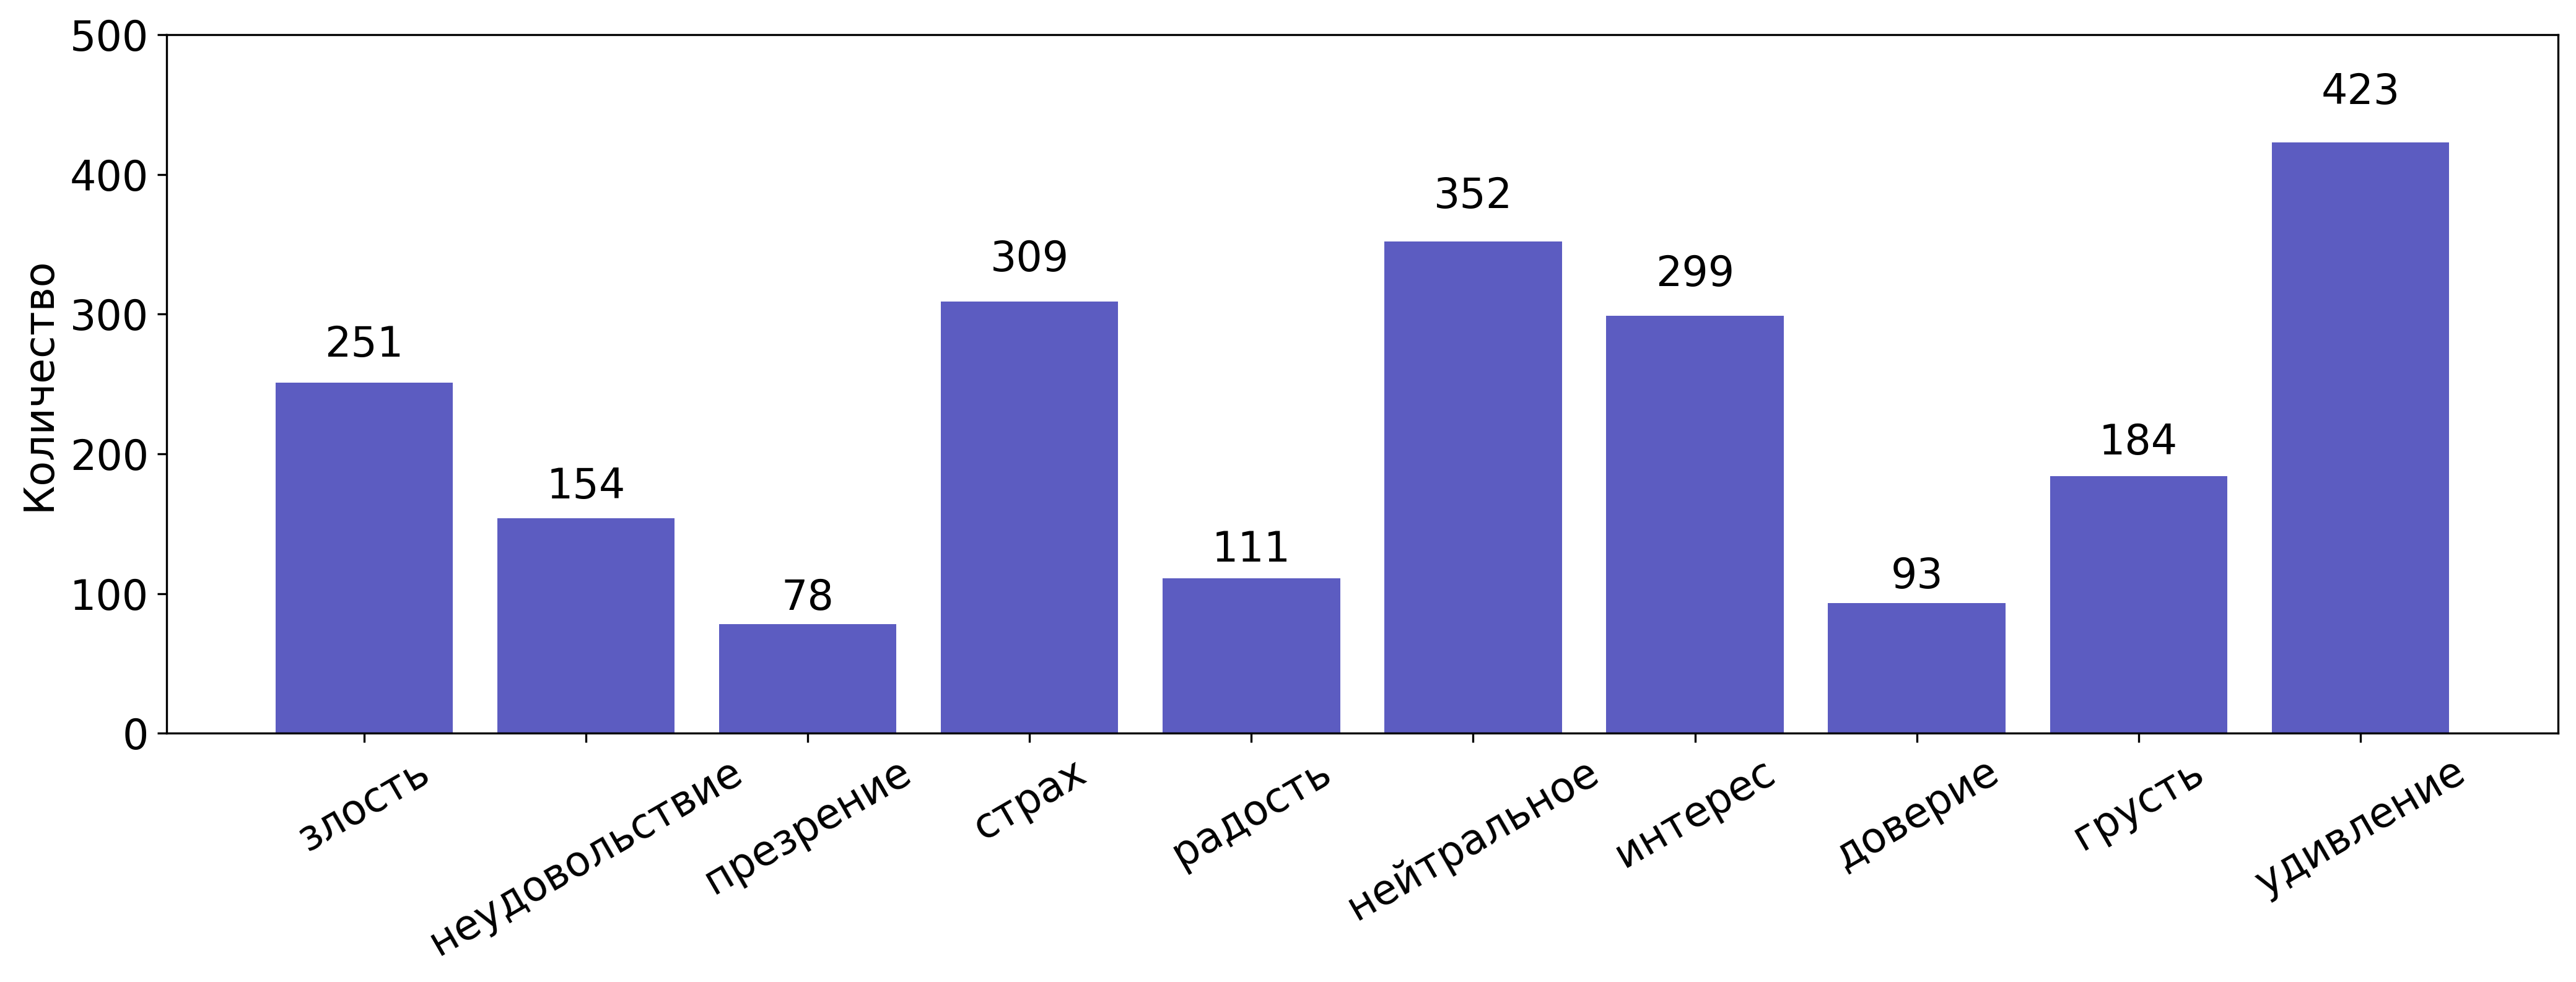
\includegraphics[scale=0.45]{class_distribution.png}
    \caption{Распределение классов в итоговом наборе данных}
    \label{fig:class_distribution}
\end{figure}

\subsection{Модели классификации}

\subsubsection{Предобработка текстов}

Чтобы работать с текстами, сначала их нужно нормализовать. Этот процесс включает несколько этапов.

\bigskip
\begin{enumerate}
 \item приводим текст к нижнему регистру;
 \item удаляем все <<не слова>> и <<стоп-слова>>;
 \item лемматизируем текст.
\end{enumerate}

\bigskip
Вот пример обработки небольшого текста:

\bigskip
\fbox{Квартира простояла пустой и запечатанной только неделю.} $\to$ \fbox{квартира простаивать пустой запечатывать неделя}


\subsubsection{Представление предложений}


Теперь текст нужно перевести в векторное пространство $R^n$, где $n$ --- размерность признаково пространства используемой модели. Пусть текст $D$ состоит из слов $d \in D$, $f$ --- модель, строящая отображение пространства слов в векторное пространство действительных чисел $f(d) \to R^n$. Тогда текст для классификатора выглядит так:

\begin{equation*}
 \frac{1}{\#D}\sum_{d \in D} f(d) \in R^n
\end{equation*}

В этой работе использованы модели предобученные на корпусе русскоязычных текстов <<Тайга>>:

\bigskip
\begin{itemize}
 \item word2vec \& skip-gram: \textit{tayga\_upos\_skipgram\_300\_2\_2019} ($n = 300$);
 \item ELMo: \textit{tayga\_lemmas\_elmo\_2048\_2019} ($n = 2048$).
\end{itemize}

\bigskip
Особенность применения ELMo заключается в том, что берется среднее значение всех слоев для каждого слова.

\subsection{Архитектура моделей классификации}

Для классификации были выбраны алгоритмы классического машинного обучения:

\bigskip
\begin{itemize}
 \item случайный лес (Random Forest);
 \item логистическая регрессия (Logistic Regression);
 \item метод опорных векторов (Support Vector Machine).
\end{itemize}

\bigskip
Схематично модели классификации представлены на рис. \ref{fig:models}.

\begin{figure}[ht]
    \centering
    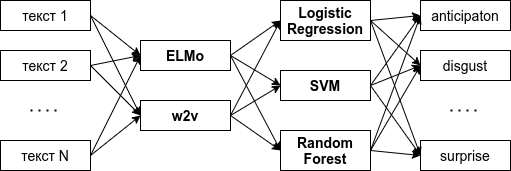
\includegraphics[scale=0.6]{models.png}
    \caption{Архитектура моделей классификации}
    \label{fig:models}
\end{figure}


\subsection{Эксперименты}


Для эмоциональной модели Роберта Плутчика результаты получились следующие:

\bigskip
\begin{table}[ht]
\caption{Значения Macro F1 меры}
\label{tab:plutchik}
\centering
\begin{tabular}{ccccc}
Macro F1 & \textbf{log reg} & \textbf{SVM} & \textbf{random forest} & \textbf{tuned random forest}\\
\textbf{w2v} & 0.21519548 & 0.27992996 & 0.23415391 & 0.23932876\\
\textbf{ELMO} & 0.25900211 & 0.32828541 & 0.31197309 & 0.43861588
\end{tabular}
\end{table}


Для эмоциональной модели Пола Экмана:

\bigskip
\begin{table}[ht]
\caption{Значения Macro F1 меры}
\label{tab:ekman}
\centering
\begin{tabular}{ccccc}
Macro F1 & \textbf{log reg} & \textbf{SVM} & \textbf{random forest} & \textbf{tuned random forest}\\
\textbf{w2v} & 0.25493596 & 0.18245115 & 0.21223037 & 0.37710993 \\
\textbf{ELMO}& 0.20242784 & 0.3007757 & 0.34183484 & 0.42405119
\end{tabular}
\end{table}









































% \label{chapter:OptimalBeamDesign}
% \thispagestyle{fancy}
%
%
% \par
%
%
%
% Наконец, в \,\ref{section:NumericalMethod:AuxiliaryProblem}, \ref{section:NumericalMethod:EVP}
% обсуждаются численные аспекты решения задачи о свободных колебаниях балки.
% Предлагается численный алгоритм градиентного типа решения задачи.
%
%
%
% Приводятся и анализируются полученные результаты вычислительных экспериментов.
%
%
%
% \bigskip
% \par
% Для практической реализации использовались:
% \begin{enumerate}
% \item Язык Python 3.7.2
% \item Библиотеки расширения для Python: matplotlib 3.0.3, numpy 1.16.1.
% \item Среда разработки visual studio code 1.34.1
% \item PyQt 5.12.1 используется для графической состовляющей модуля
% \end{enumerate}
%
%
%
%
% \par
% Библиотека "numpy" - это библиотека языка Python, добавляющая поддержку больших многомерных массивов и матриц, а так же большую библиотеку высокоуровневых математических функций для операций с этими массивами. Используется как необходимая библиотека для matplotlib
%
%
%
% \bigskip
% \par
% Библиотека "matplotlib" - это библиотека двумерной графики для языка програмирования Python, с помощью которой можно создавать высококачественные рисункиразличных форматов. Используется вывода графиков.
%
%
%
% \bigskip
% \par
% PyQt --- набор «привязок» графического фреймворка Qt для языка программирования Python, выполненный в виде расширения Python.
%
%
%
% \section{Численный метод решения краевой задачи для уравнения $(ay'')'' = f$}
\label{section:NumericalMethod:AuxiliaryProblem}
%
%
%
\begin{equation}
\label{DE:4Order:F}
(ay'')'' = f
\end{equation}
%
%
%
\par
Для численного решения задачи
\eqref{DE:4Order:F}
с соответствующими краевыми условиями
будем использовать метод \textbf{\emph{матричной прогонки}}.
%
%
%
Для этого уравнение
\eqref{DE:4Order:F}
представим в виде следующей системы дифференциальных уравнений второго порядка:
\begin{equation}
\begin{cases}
y''(x) = \displaystyle \frac{z(x)}{a(x)},
\\
z''(x) = f(x),
\end{cases}
\qquad
x \in I.
\end{equation}
%
%
%
%
%
\par
Введем на отрезке
\(0 \le x \le 1\)
разностную сетку с постоянным шагом \(H\).
%
%
%
Узлы этой сетки будем обозначать через
\(x_k = kH\),
где
\(k = 0, 1, \ldots, N\).
%
%
%
В свою очередь,
значения функций
\(y(x), z(x), a(x), f(x)\)
в узлах
будем обозначать через
\(y_k, z_k, a_k, f_k\)
соответственно.
%
%
%
 Функцию \(y(x)\) будем аппроксимировать разложив в ряд Тейлора слева \(y(x-h)\) и справа \(y(x+h)\) следующим видом
	\begin{equation*}
	y(x+h)=y(x) + \frac{y'(x)h}{1!} + \frac{y''(x)h^2}{2!} + \frac{y'''(x)h^3}{3!} + \ldots
	\end{equation*}
	\begin{equation}
	y(x-h)=y(x) - \frac{y'(x)h}{1!} + \frac{y''(x)h^2}{2!} - \frac{y'''(x)h^3}{3!} + \ldots
	\end{equation}
	На выходе получаем следующее
	\begin{equation*}
	y(x+h)+y(x-h) = 2y(x)+y''(x)h^2 \quad \Rightarrow
	\end{equation*}
	\begin{equation}
	\frac{y_{k+1}-2y_k+y_{k-1}}{h^2}=y''(x_k)=\frac{z_k}{U_k}
	\end{equation}
	Аналогично выполняем аппроксимацию \(z(x)\)
	\begin{equation}
	\frac{z_{k+1}-2z_k+z_{k-1}}{h^2}=f(k)
	\end{equation}
	Для дальнейшей матричной прогонки определим вектор
	\(X_k= \left( \begin{matrix}
	y_k\\z_k
	\end{matrix} \right)\) 
	и коэффициенты \(A_k,B_k,C_k\).
	\begin{equation}
	A_kX_{k+1}-B_kX_k+C_kX_{k-1}=F_k, \quad k=1\ldots N-1
	\end{equation}
	Выпишем полученную систему уравнений:
	\begin{equation}
	\begin{cases}
	y_{k+1}-2y_k+y_{k-1} - \frac{z_kh^2}{U_k}=0 \\
	z_{k+1}-2z_k+z_{k-1}=f(k)h^2 \\
	F_k= \left( \begin{matrix}
	0\\f(k)h^2
	\end{matrix} \right)
	\end{cases}
	\end{equation}
	Выразим матричное уравнение и выразим коэффициенты \(A_k,B_k,C_k\)
	\begin{equation*}
	\left( \begin{matrix}
	1&0\\0&1
	\end{matrix} \right)X_{k+1}-\left( \begin{matrix}2&\frac{h^2}{U_k}\\0&2\end{matrix}\right)X_k+
	\left( \begin{matrix}1&0\\0&1\end{matrix}\right)X_{k-1}=F_k
	\end{equation*}
	\begin{equation}\label{eq4}
	A_k=\left( \begin{matrix}1&0\\0&1\end{matrix} \right) \quad 
	B_k=\left( \begin{matrix}2&\frac{h^2}{U_k}\\0&2\end{matrix} \right) \quad 
	C_k=\left( \begin{matrix}1&0\\0&1\end{matrix} \right), \quad  A_k=C_k=E
	\end{equation}
	Для определения коэффициентов \(X_k\)~- необходимо рассмотреть обратный итерационный процесс
	\begin{equation}\label{eq5}
	X_k=L_{k+1}X_{k+1}+M_{k+1}
	\end{equation}
	Выведем формулы для коэффициентов \(L_k\) и \(M_k\)
	\begin{equation*}
	A_kX_{k+1}-B_kX_k+C_k(L_kX_k+M_k)=F_k
	\end{equation*}
	\begin{equation*}
	A_kX_{k+1}+X_k(C_kL_k-B_k)=F_k-C_kM_k
	\end{equation*}
	\begin{equation*}
	X_k=-(C_kL_k-B_k)^{-1}A_kX_{k+1}+(C_kL_k-B_k)^{-1}(F_k-C_kM_k)
	\end{equation*}
	\begin{equation}\label{eq6}
	L_{k+1}=-(C_kL_k-B_k)^{-1}A_k
	\end{equation}
	\begin{equation}\label{eq7}
	M_{k+1}=(C_kL_k-B_k)^{-1}(F_k-C_kM_k)
	\end{equation}
	Рассмотрим алгоритм метода матричной прогонки для трех возможных способов закрепления балки.
	
	\bigskip\quad Алгоритм:
	\begin{enumerate}
		\item Вычисляем коэффициенты \(A_k,B_k,C_k\) по формулам (\ref{eq4}) для\\ k=1\ldots N-1
		\item Определяем граничные условия метода в соответствии с типом закрепления балки:
		\begin{enumerate}
			\item Балка свободно оперта на обоих концах свей длины.
			
			В данном случае краевыми условиями на обои концах \((x=0,x=l)\) являются следующие условия:
			\begin{equation*}
			y=y''=0|_{x=0}, \quad y=y''=0|_{x=l}
			\end{equation*}
			Исходя из этого, получим:
			\begin{equation*}
			L_0=\left( \begin{matrix}0&0\\0&0\end{matrix} \right),\quad
			M_0=\left( \begin{matrix}0\\0\end{matrix} \right),
			\end{equation*}
			\begin{equation*}
			L_n=\left( \begin{matrix}0&0\\0&0\end{matrix} \right),\quad
			M_n=\left( \begin{matrix}0\\0\end{matrix} \right),\quad,
			X_n=\left( \begin{matrix}0\\0\end{matrix} \right)
			\end{equation*}
			\item Балка жестко закреплена на обоих концах.\\
		
			
			В данном случае краевыми условиями на обоих концах \\\((x=0,x=l)\) являются следущие условия:
			\begin{equation*}
			y=y'=0|_{x=0}, \quad y=y'=0|_{x=l}
			\end{equation*}
			Исходя из этого, получим:
			\begin{equation*}
			L_0=\left( \begin{matrix}0&0\\\frac{2U_0}{h^2}&0\end{matrix} \right),\quad
			M_0=\left( \begin{matrix}0\\0\end{matrix} \right),
			\end{equation*}
			Вычислим \(X_n\):
			\begin{equation*}
			X_{n-1}=L_nX_n+M_n,\quad y_{n-1}=\frac{h^2z_n}{2U_0};
			\end{equation*}
			\begin{equation*}
			X_{n-1}=\left(\begin{matrix}0&\frac{h^2}{2U_0}\\0&0\end{matrix}\right)\left(\begin{matrix}y_n\\z_n\end{matrix}\right)+\left(\begin{matrix}0\\0\end{matrix}\right);
			\end{equation*}
			\begin{equation*}
			\left(\begin{matrix}l_{11}&l_{12}\\l_{21}&l_{22}\end{matrix}\right)\left(\begin{matrix}y_n\\z_n\end{matrix}\right)+\left(\begin{matrix}m_1\\m_2\end{matrix}\right)=\left(\begin{matrix}0&\frac{h^2}{2U_0}\\0&0\end{matrix}\right)\left(\begin{matrix}y_n\\z_n\end{matrix}\right);
			\end{equation*}
			\begin{equation*}
			\left(\begin{matrix}l_{11}&l_{12}-\frac{h^2}{2U_0}\\l_{21}&l_{22}\end{matrix}\right)\left(\begin{matrix}y_n\\z_n\end{matrix}\right)=\left(\begin{matrix}m_1\\m_2\end{matrix}\right);
			\end{equation*}
			\begin{equation*}
			X_n=-\left(\begin{matrix}l_{11}&l_{12}-\frac{h^2}{2U_0}\\l_{21}&l_{22}\end{matrix}\right)^{-1}\left(\begin{matrix}m_1\\m_2\end{matrix}\right);
			\end{equation*}
			\item Балка жестко закреплена на одном конце и оперта на другом.
					
			В данном случае краевыми условиями на обои концах \((x=0,x=l)\) являются следующие условия:
			\begin{equation*}
			y=y'=0|_{x=0}, \quad y=y'=0|_{x=l}
			\end{equation*}
			Исходя из этого, получим:
			\begin{equation*}
			L_0=\left( \begin{matrix}0&0\\\frac{2U_0}{h^2}&0\end{matrix} \right),\quad
			M_0=\left( \begin{matrix}0\\0\end{matrix} \right),
			\end{equation*}
			\begin{equation*}
			X_N=\left( \begin{matrix}0\\0\end{matrix} \right).
			\end{equation*}
		\end{enumerate}
		\item Вычисляем  коэффициенты \(L_k,M_k\) по формулам (\ref{eq6}) и (\ref{eq7}) для\\ k=1\ldots N-1.
		\item Начиная с \(k=N-1~\text{до}~k=0~\text{вычисляем векторы}~X_k\) по формуле (\ref{eq5}). 
		\item Получив значения \(X-k\), получаем значения \(y_k\text{ и } z_k\).
	\end{enumerate}

%
% Численный метод определения собственной пары %%%
% \section{Численный метод решения задачи о поперечных колебаниях балки}
\label{section:NumericalMethod:EVP}

\begin{equation*}  
(Uy'')''=\lambda Vy
\end{equation*}
Полученное решение краевой задачи  \(y_{(n)}\) используем для определения следующего приближения безрезонансного интервала:
\begin{equation*}  
(Uy_{(n+1)}'')''=f=Vy_{(n)}
\end{equation*}
%
%
%
%
Вариационное представление
\eqref{FirstEigenvalue:VariationalPrinciple}
первого собственного значения $\lambda_1[u]$
определяем следущим \emph{\textbf{отношением Рэлея}}:
%
%
%
%
\begin{equation*}  
\lambda_1^{(n)}=\frac{\int_{0}^{1}Uy_{(n)}''^2dx}{\int_{0}^{1}Vy_{(n)}^2dx},
\end{equation*}
\begin{equation*}  
Uy_{(n)}''^2=\frac{1}{U}(Uy_{(n)}''^2)^2=\frac{1}{U}z^2,
\end{equation*}
\begin{equation}\label{eq9}   
\lambda_1^{(n)}=\frac{\int_{0}^{1}\frac{1}{U}z_{(n)}^2dx}{\int_{0}^{1}Vy_{(n)}^2dx}.
\end{equation}


Решение уравнения (\ref{eq9}) находим методом трапеций\\
\begin{equation}\label{eq10} 
\int_a^bf(x)\approx\frac{h}{2}(f(x_0)+2\sum\limits_{i=1}^{n-1} f(x_i) +f(x_n),
\end{equation}
\begin{equation*}  
h=\frac{b-a}{n}=1 \quad  x_i=a+ih \quad  i=0,1\ldots n,
\end{equation*}
\begin{center}  
\(i=0 \quad x_0+0*1\quad \Rightarrow\quad f(x_0)=Vy^2\bigg|_0\)\\
\(i=1 \quad x_1+1*1\quad \Rightarrow\quad f(x_1)=Vy^2\bigg|_1\)\\
\ldots\\
\ldots\\
\(i=n \quad x_n+1*n\quad \Rightarrow\quad f(x_n)=Vy^2\bigg|_n\)
\end{center}
\par
Далее заносим значения под знак суммы (\ref{eq10}) и находим все собственные значения $\lambda_1[u]$ описывающее резонансное поведение в процессе колебания балки, в этом случае следующая погрешность и является показательной
\begin{equation*}  
|\lambda_1^{(n+1)} + \lambda_1^{(n)}|<\varepsilon\approx 10^{10}.
\end{equation*}
%
% Поиск седловой точки %%%
% \section{Поиск седловой точки}


\par
Оптимальное решение $w$ и соответствующая ему собственная функция $y_1$ образуют седловую точку функционала 
\begin{equation}
F(u,z) = \frac{\int_{0}^{1}eu^{\nu}z''^2  \, dx}{\int_{0}^{1}\rho uz^2 \, dx},
\end{equation}
т.\,е. выполняются неравенства
\begin{equation}
F(u,y_1) \leq F(w,y_1) \leq F(w,z),
\end{equation}
где $u$ и $z$ пробегают допустимые множества.
%
\bigskip
\par
Седловую точку ищем с помощью следущей процедуры: 
%
\par 
\begin{enumerate}
	\item задается начальное приближение $u_0 \in U$;
	%
	\item  для заданного $u_n$ решается задача на собственные значения для определения собственной пары ($\lambda_1[u_n], y_1[u_n]$);
	%Это эквивалентно решению задачи на собственные значения.
	
	\par
	%
	\item находится новое приближение $u_{n+1}$, для которого
	\begin{equation}
	F(u_{n+1},y_1[u_n]) = \max_{u \in U} F(u,y_1[u_n]);
	\end{equation}
	
	\item если 
	\begin{equation}
	|\lambda_1[u_{n+1}] - \lambda_1[u_{n}]| < \varepsilon,
	\end{equation}
	где $\varepsilon$~--- заданная  точность, то итерационная процедура завершается, а $u_{n+1}$ выступает в качестве оптимального распределения.
	\bigskip
	\par
	В противном случае переходим к шагу 2 с $n=n+1$.
\end{enumerate}

\bigskip
\par
После определения собственной пары составляем уравнение максимизации колебательного процесса упругой балки, для определения нового оптимального приближения, с последующим определением новой собственной пары, для продолжения итерационного процесса
\begin{equation}
\label{MaximizingVibrating} 
e\xi y''^2_n - \lambda\rho\xi y^2_n + \mu\xi \rightarrow \max,
\end{equation}

\begin{equation*}
\begin{aligned}
\int_0^1{eU_{n+1}y''^2_ndx} - \lambda_n\int_0^1{\rho U_{n+1}y^2_ndx}\geqslant	\\
\geqslant \int_0^1{eU_ny''^2_ndx} - \lambda_n\int_0^1{\rho U_ny^2_ndx}\\
\end{aligned}
\end{equation*}

\begin{equation*} 
e(x)\xi y''^2_n - \lambda\rho(x)\xi y^2_n + \mu\xi \rightarrow \max.
\end{equation*}
%
%
%
Подставляем $\mu$  и для каждого x, решим задачу получив $\xi(x)$,
%
%
%
\begin{equation*} 
\xi(e(x) y''^2_n - \lambda\rho(x)\xi y^2_n + \mu) \rightarrow \max,
\end{equation*}
$\mu$ надо подобрать так, чтоб интеграл $\int_0^1{\xi(x)dx} = 1$ был равен единице, вводим следующую функцию: 
\begin{equation*} 
f(\mu)=\int_0^1{\xi_{\mu}(x)dx} - 1,
\end{equation*}
\begin{equation*} 
\xi \in [\alpha,\beta] \qquad \xi(x) \rightarrow \max,
\end{equation*}
%
%
%
где $\alpha , \beta$~--- ограничения на площадь, $\alpha= u_{min}$, $\beta= u_{max}$ 
%
%
%
\begin{center}
$$ (\lambda_n,y_n) \rightarrow \xi(x)= U_{n+1},$$
$$ (\lambda_{n+1},y_{n+1}) \rightarrow \xi(x)= U_{n+2},$$
\ldots \\
\ldots \\
$$(\lambda_{n+k-1},y_{n+k-1}) \rightarrow \xi(x)= U_{n+k};$$
\end{center}
%
%
%
%
Для решения оптимизационной поточечной задачи, использем метод секущих Ньютона (не требующий производную функции) находим ноль функции, и задача \eqref{MaximizingVibrating} принимает следущий вид
%
%
%
%
\begin{equation*} 
f(\mu)=\int_0^1{\xi_{\mu}(\frac{ez^2_n}{u^2\rho^2}+\lambda\rho y^2_n+\mu)dx} - 1
\end{equation*}
%
%
метод секущих для следующей итерации $x_n$
%
%
\begin{equation*} 
x_n=x_{n-1} - f(x_n -1) \frac{x_{n-1}-x_{n-2}}{f(x_{n-1})-f(x_{n-2})}=\frac{x_{n-2}f(x_n-1)-x_{n-1}f(x_{n-2})}{f(x_{n-1}-f(x_{n-2}))}.
\end{equation*}
Для первого выполнения итерации берем  $x_{n-1}$~--- значения первичной собственной пары $x_{n-2} = 0$. Задача на собственные значения решается многократно, останавливается когда $|\lambda_{n+1}-\lambda_n| <\varepsilon\approx 10^{5}$

%О том как ищешь седловую точку.

%Поточечная задача оптимизации от $\xi$ и т.д.

%Как решаешь эту задачу.

%
% РЕЗУЛЬТАТЫ ВЫЧИСЛИТЕЛЬНОГО ЭКСПЕРИМЕНТА %%%
% \section{Результаты вычислительного эксперимента}
%
%
%
%
\par
Примененные численные методы демонстрировали сходимость к оптимальному решению балки, с определением формы балки и частоты безрезонансных колебаний балки, с учетом заданных параметров проектирования (толщины, массы), при ограничении на толщину.
%
%
%
\begin{enumerate}
	\item 	$h(x) = 2\sqrt{x}$; \;\; $u_{min} = 0{,}4$; \;\; $u_{max} = 1{,}8$
	\item 	$h(x) = 181.263 \rho^2e/x^6 $; \;\; $u_{min} = 0{,}4$; \;\; $u_{max} = 1{,}8$
\end{enumerate}

\begin{center}
	\begin{figure}
		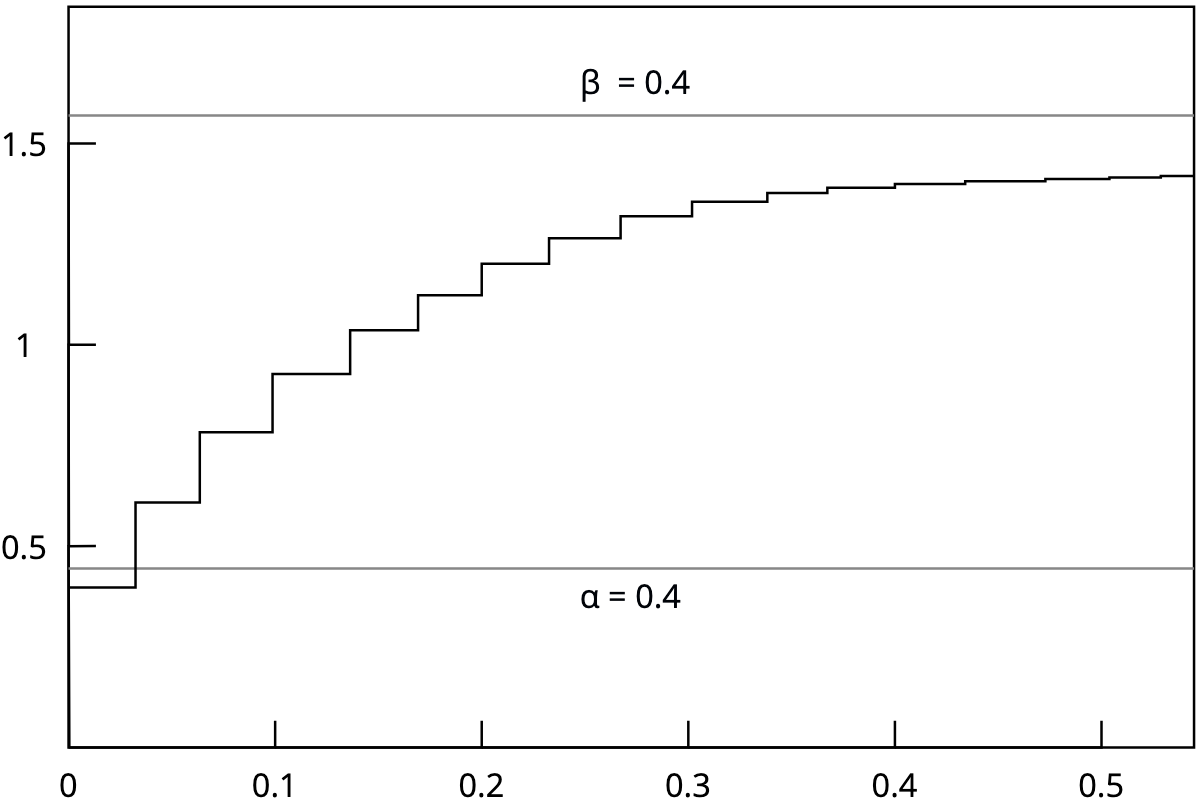
\includegraphics[width=1\linewidth]{untitled2.png}
		\caption{Оптимальное распределение толщины балки $u_{opt}$ (1).}
		\bigskip
		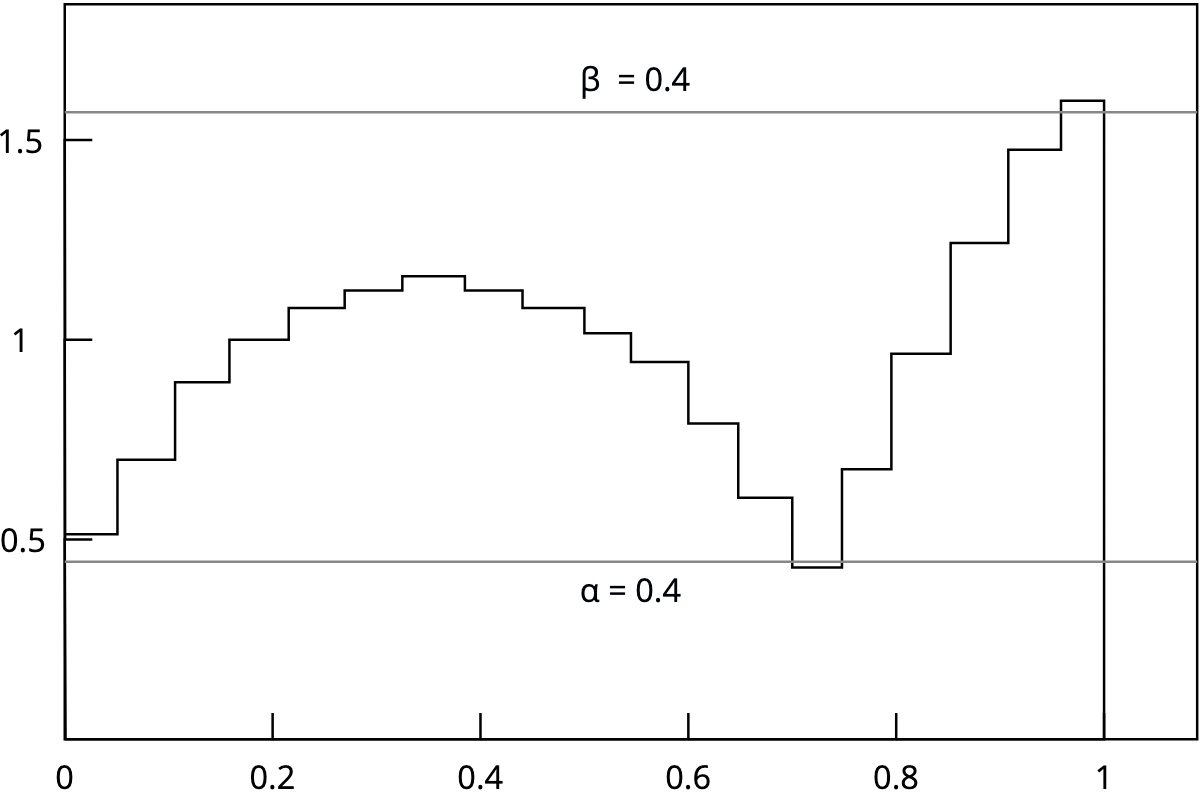
\includegraphics[width=1\linewidth]{untitled.png}
		\caption{Оптимальное распределение толщины балки $u_{opt}$ (2).}
	\end{figure}
	%
	%
	%
\end{center}



%Картинки.

%При каких параметрах получены.

%Каков эффект оптимизации.

%Анализ.

%Параметры $\alpha, \beta, \nu$.

%Оптимальное распределение
%Оптимизация эффективность




%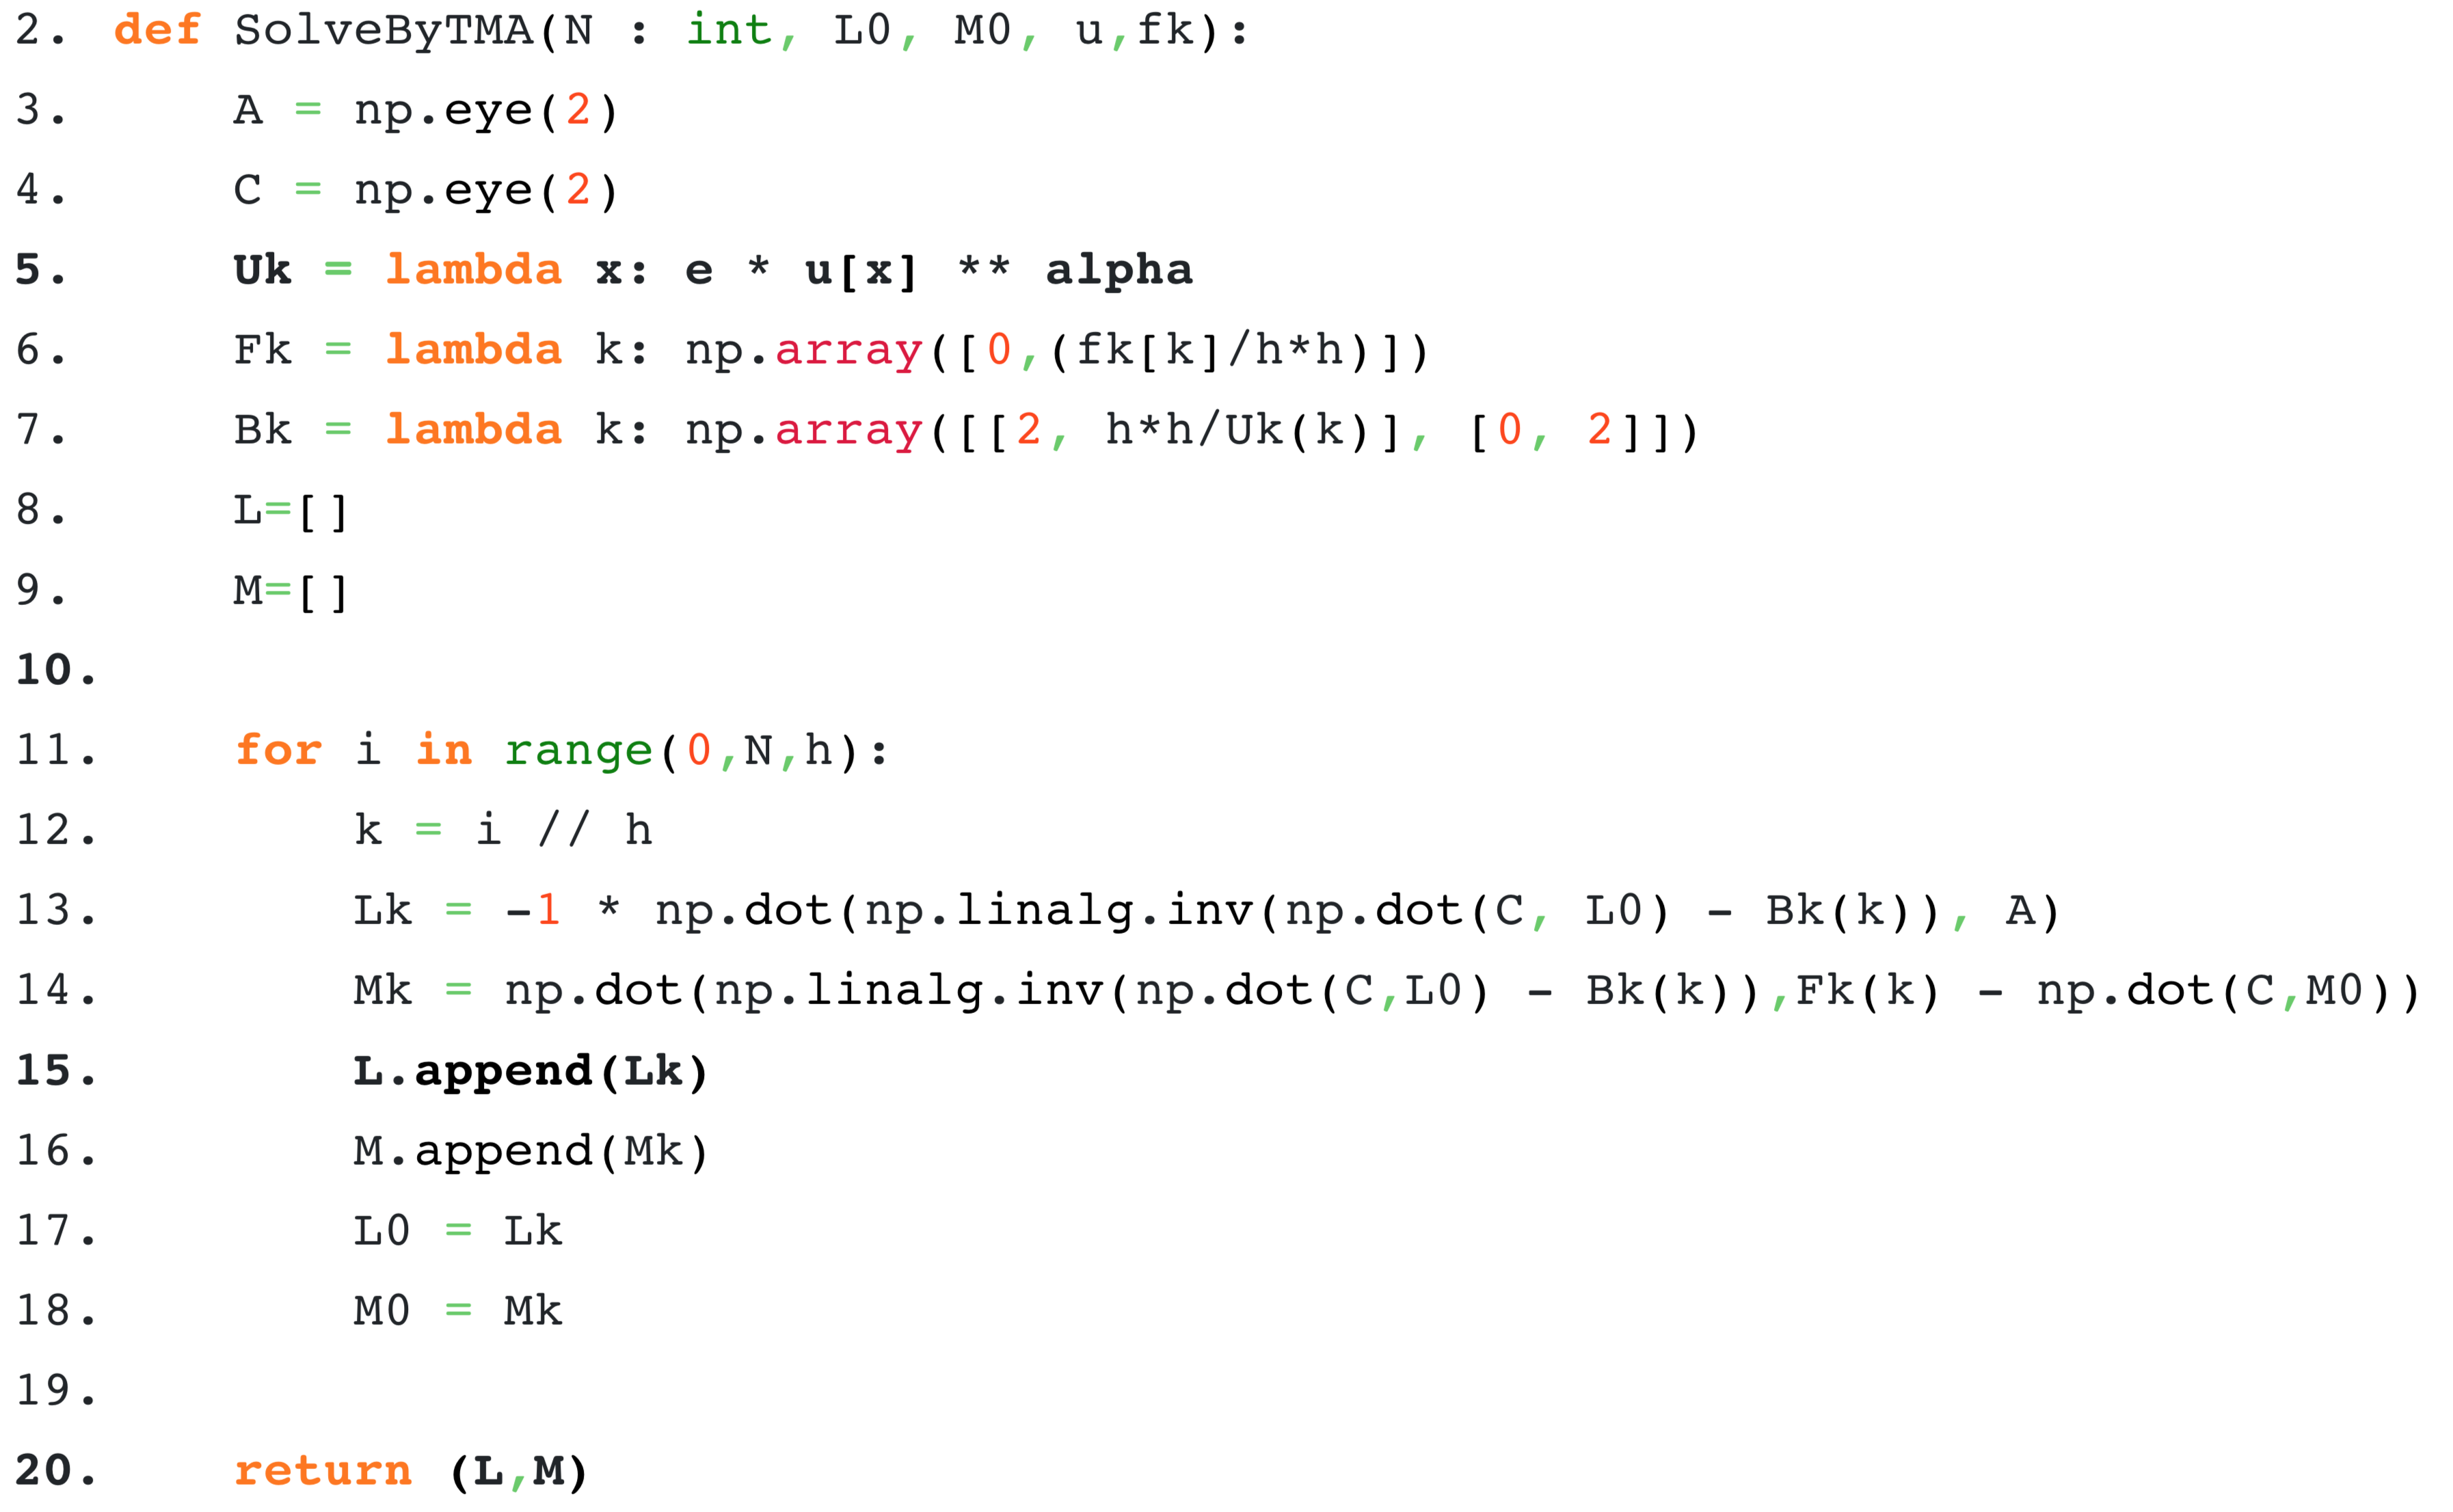
\includegraphics[width=0.5\linewidth]{1code.png}
%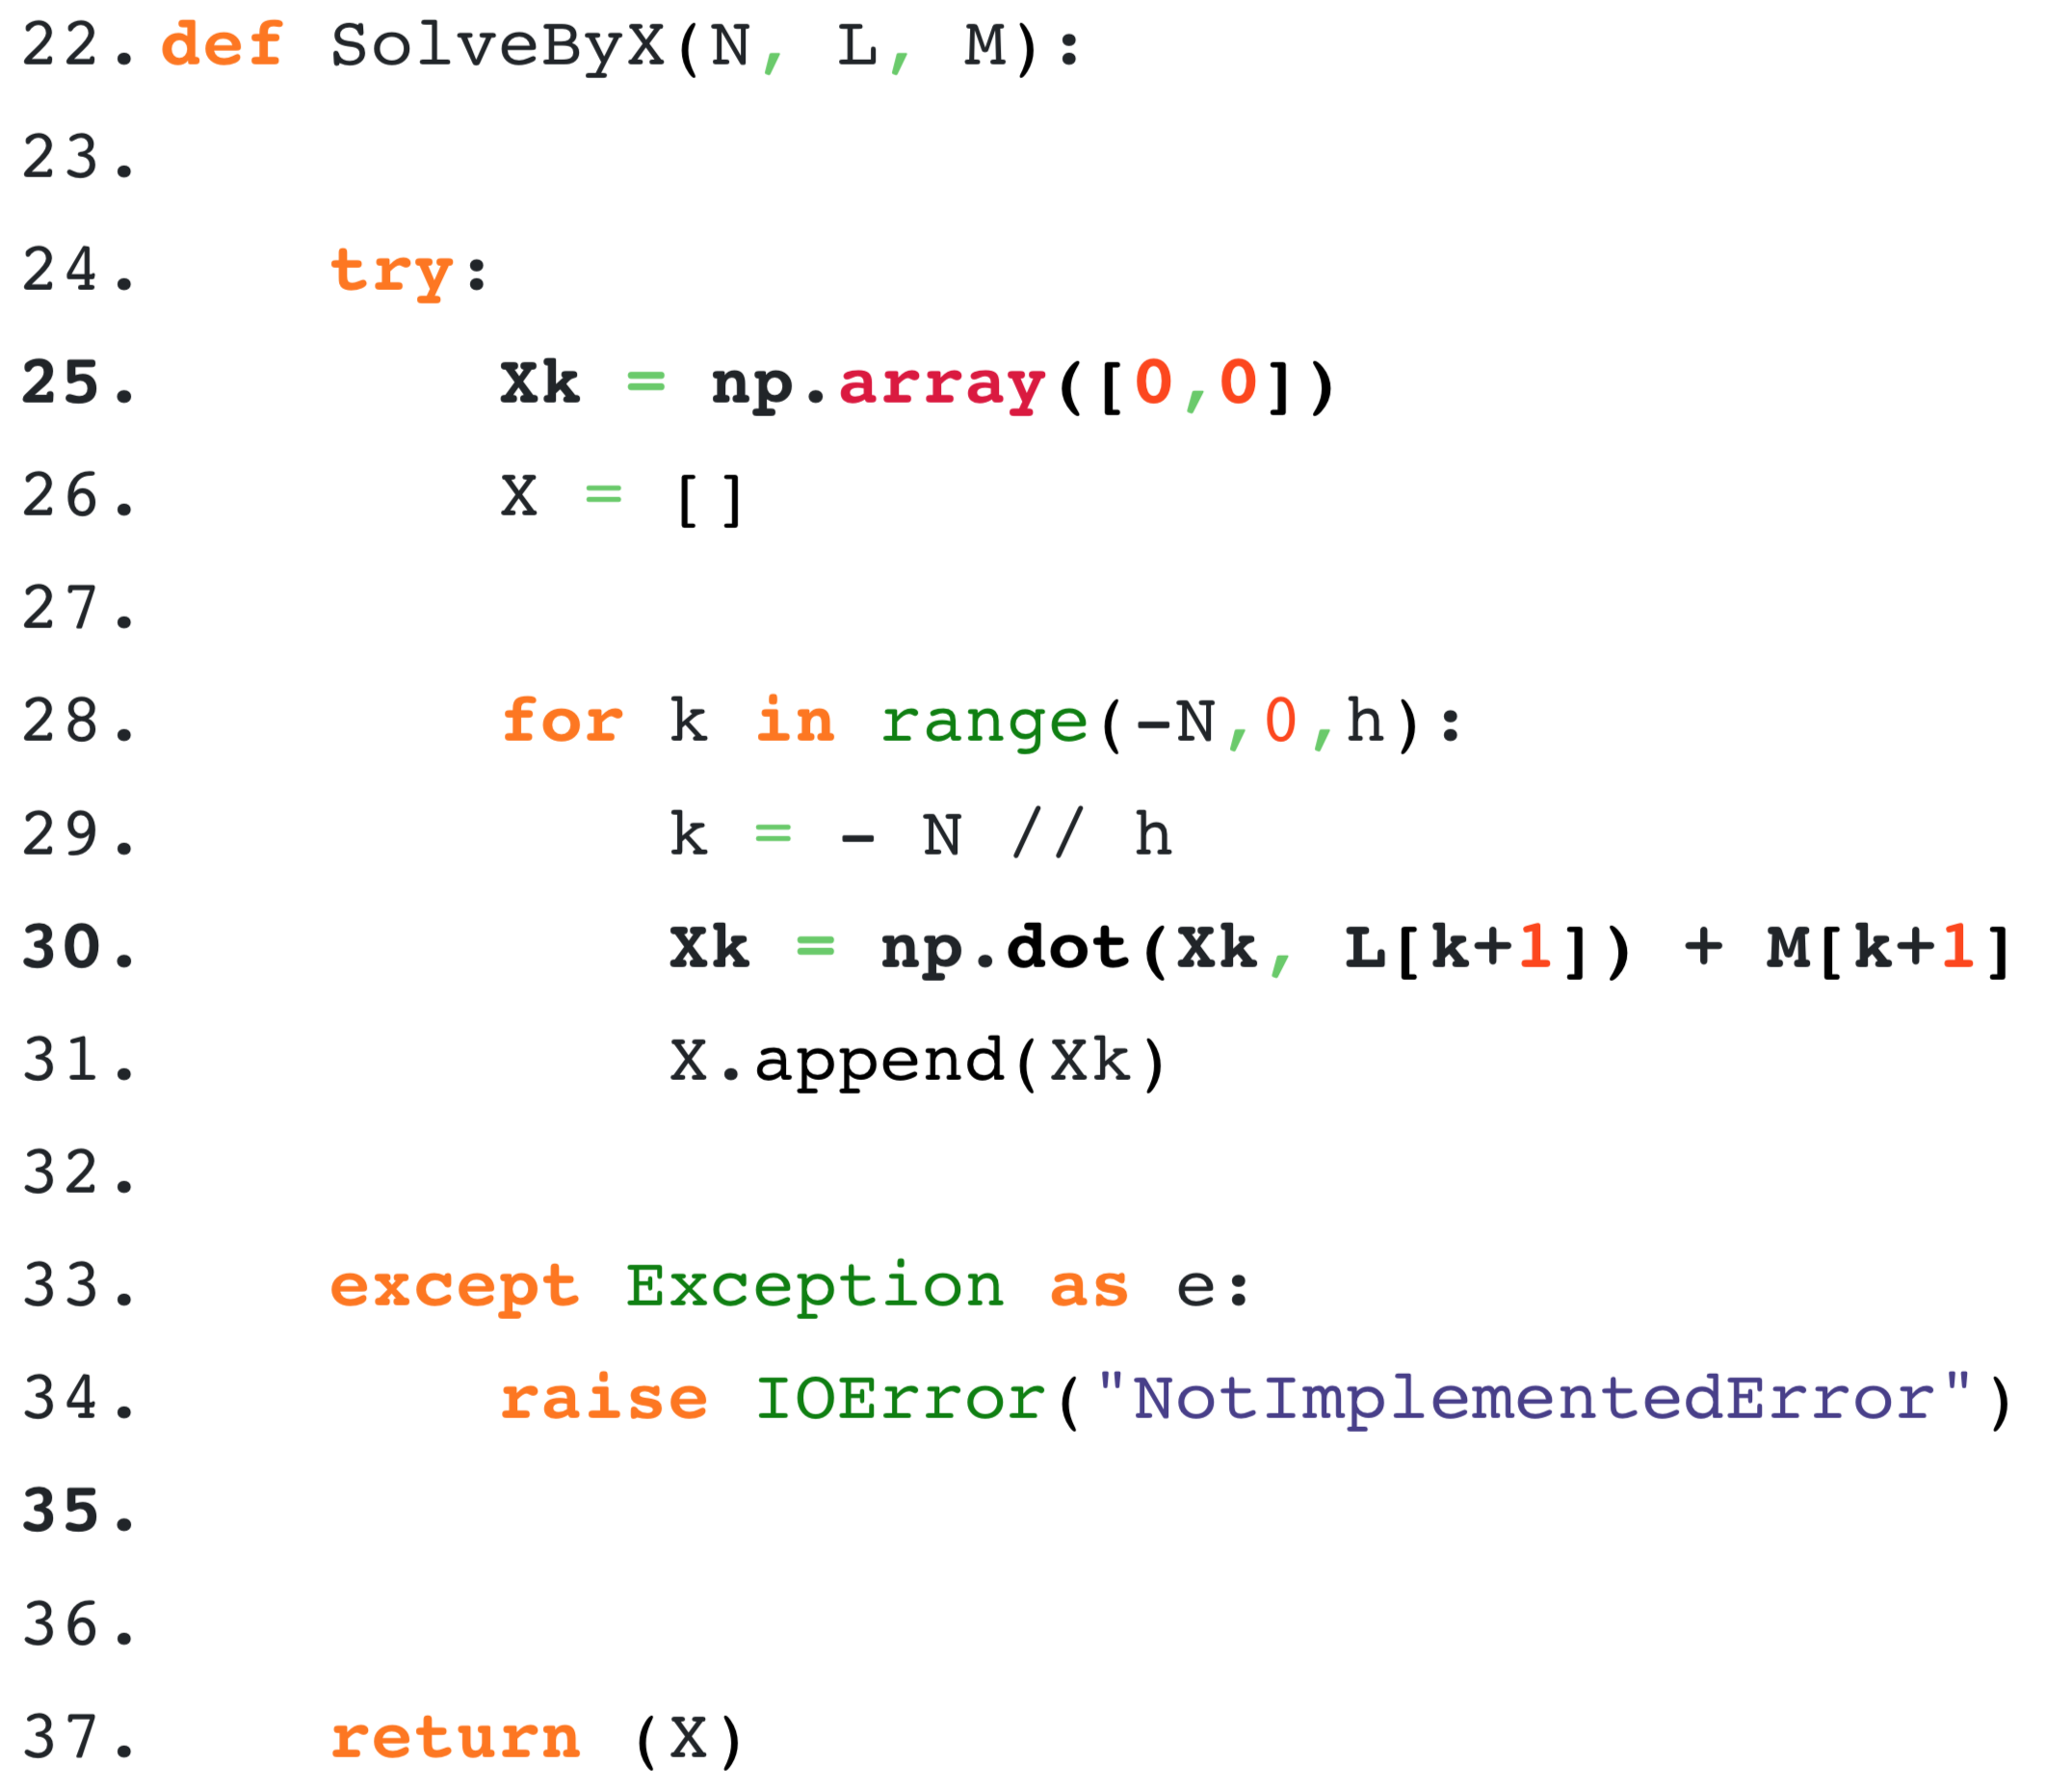
\includegraphics[width=0.5\linewidth]{2code.png}
%\\
%При каких параметрах получены.
%
%Каков эффект оптимизации.
%
%Анализ.
%
%Параметры $\alpha, \beta, \nu$.
